%% Copyright (c) 2002, 2010 Sam Williams
%% Copyright (c) 2010 Richard M. Stallman
%% Permission is granted to copy, distribute and/or modify this
%% document under the terms of the GNU Free Documentation License,
%% Version 1.3 or any later version published by the Free Software
%% Foundation; with no Invariant Sections, no Front-Cover Texts, and
%% no Back-Cover Texts. A copy of the license is included in the
%% file called ``gfdl.tex''.


\chapter{A Stark Moral Choice}

On September 27, 1983, computer programmers logging on to the Usenet newsgroup net.unix-wizards encountered an unusual message. Posted in the small hours of the morning, 12:30 a.m. to be exact, and signed by \url{rms@mit-oz}, the message's subject line was terse but attention-grabbing. ``New UNIX implementation,'' it read. Instead of introducing a newly released version of Unix, however, the message's opening paragraph issued a call to arms:

\begin{quote}
Starting this Thanksgiving I am going to write a complete Unix-compatible software system called GNU (for Gnu's Not Unix), and give it away free to everyone who can use it. Contributions of time, money, programs and equipment are greatly needed.\endnote{See Richard Stallman, ``Initial GNU Announcement'' (September 1983).}
\end{quote}

To an experienced Unix developer, the message was a mixture of idealism and hubris. Not only did the author pledge to rebuild the already mature Unix operating system from the ground up, he also proposed to improve it in places. The new GNU system, the author predicted, would carry all the usual components -- a text editor, a shell program to run Unix-compatible applications, a compiler, ``and a few other things.''\endnote{\textit{Ibid.}} It would also contain many enticing features that other Unix systems didn't yet offer: a graphic user interface based on the Lisp programming language, a crash-proof file system, and networking protocols built according to MIT's internal networking system.

``GNU will be able to run Unix programs, but will not be identical to Unix,'' the author wrote. ``We will make all improvements that are convenient, based on our experience with other operating systems.''

Anticipating a skeptical response on some readers' part, the author made sure to follow up his operating-system outline with a brief biographical sketch titled, ``Who am I?'':

\begin{quote}
I am Richard Stallman, inventor of the original much-imitated EMACS editor, now at the Artificial Intelligence Lab at MIT. I have worked extensively on compilers, editors, debuggers, command interpreters, the Incompatible Timesharing System and the Lisp Machine operating system. I pioneered terminal-independent display support in ITS. In addition I have implemented one crashproof file system and two window systems for Lisp machines.\endnote{\textit{Ibid.}}
\end{quote}

As fate would have it, Stallman's fanciful GNU Project missed its Thanksgiving launch date. By January, 1984, however, Stallman made good on his promise and fully immersed himself in the world of Unix software development. For a software architect raised on ITS, it was like designing suburban shopping malls instead of Moorish palaces. Even so, building a Unix-like operating system had its hidden advantages. ITS had been powerful, but it also possessed an Achilles' heel: MIT hackers had written it specifically to run on the powerful DEC-built PDP-10 computer. When AI Lab administrators elected to phase out the lab's PDP-10 machine in the early 1980s, the operating system that hackers once likened to a vibrant city became an instant ghost town. Unix, on the other hand, was designed for portability, which made it immune to such dangers. Originally developed by junior scientists at AT\&T, the program had slipped out under corporate-management radar, finding a happy home in the cash-strapped world of academic computer systems. With fewer resources than their MIT brethren, Unix developers had customized the software to ride atop a motley assortment of hardware systems, primarily the 16-bit PDP-11 -- a machine considered fit for only small tasks by most AI Lab hackers -- but later also 32-bit mainframes such as the VAX 11/780. By 1983, a few companies, most notably Sun Microsystems, were developing a more powerful generation of desktop computers, dubbed ``workstations,'' to take advantage of that increasingly ubiquitous operating system on machines comparable in power to the much older PDP-10.

To facilitate portability, the developers of Unix had put an extra layer of abstraction between the software and the machine. Rather than writing it in the instructions of a specific machine type -- as the AI Lab hackers had done with ITS and the PDP-10 -- Unix developers wrote in a high-level language, called C. Focusing more on the interlocking interfaces and specifications that held the operating system's many subcomponents together, rather than the actual components themselves, they created a system that could be quickly modified to run on any machine. If a user disliked a certain component, the interface specifications made it possible to pull out an individual subcomponent and either fix it or replace it with something better. Simply put, the Unix approach promoted flexibility and economy, hence its rapid adoption.\endnote{See Marshall Kirk McKusick, ``Twenty Years of Berkeley Unix,'' \textit{Open Sources} (O'Reilly \& Associates, Inc., 1999): 38.}

Stallman's decision to start developing the GNU system was triggered by the end of the ITS system that the AI Lab hackers had nurtured for so long. The demise of ITS, and the AI Lab hacker community which had sustained it, had been a traumatic blow to Stallman. If the Xerox laser printer episode had taught him to recognize the injustice of proprietary software, the community's death forced him to choose between surrendering to proprietary software and opposing it.

Like the software code that composed it, the roots of ITS' demise stretched way back.  By 1980, most of the lab's hackers were working on developing the Lisp Machine and its operating system.

Created by artificial-intelligence research pioneer John McCarthy, a MIT artificial-intelligence researcher during the late 1950s, Lisp is an elegant language, well-suited for writing complex programs to operate on data with irregular structure. The language's name is a shortened version of LISt Processing. Following McCarthy's departure to the Stanford Artificial Intelligence Laboratory, MIT hackers refined the language into a local dialect dubbed MACLISP. The ``MAC'' stood for Project MAC, the DARPA-funded research project that gave birth to the AI Lab and the Laboratory for Computer Science. Led by AI Lab arch-hacker Richard Greenblatt, the AI Lab hackers during the late 1970s designed a computer specialized for running Lisp efficiently and conveniently, the Lisp Machine, then developed an entire Lisp-based operating system for it.

By 1980, two rival groups of hackers had formed two companies to manufacture and sell copies of the Lisp Machine.  Greenblatt started Lisp Machines Incorporated.  He planned to avoid outside investment and make a ``hacker company.''  Most of the hackers joined Symbolics, a conventional startup.  In 1982 they entirely ceased to work at MIT.

With few hackers left to mind the shop, programs and machines took longer to fix -- or were not fixed at all.  Even worse, Stallman says, the lab began to undergo a ``demographic change.'' The hackers who had once formed a vocal minority within the AI Lab were almost gone while ``the professors and the students who didn't really love the [PDP-10] were just as numerous as before.''\endnote{See Richard Stallman (1986).}

In 1982, the AI Lab received the replacement for its main computer, the PDP-10, which was over 12 years old. Digital's current model, the Decsystem 20, was compatible for user programs but would have required a drastic rewrite or ``port'' of ITS if hackers wanted to continue running the same operating system. Fearful that the lab had lost its critical mass of in-house programming talent, AI Lab faculty members pressed for Twenex, a commercial operating system developed by Digital. Outnumbered, the hackers had no choice but to comply.

\begin{figure}[ht] \centering
  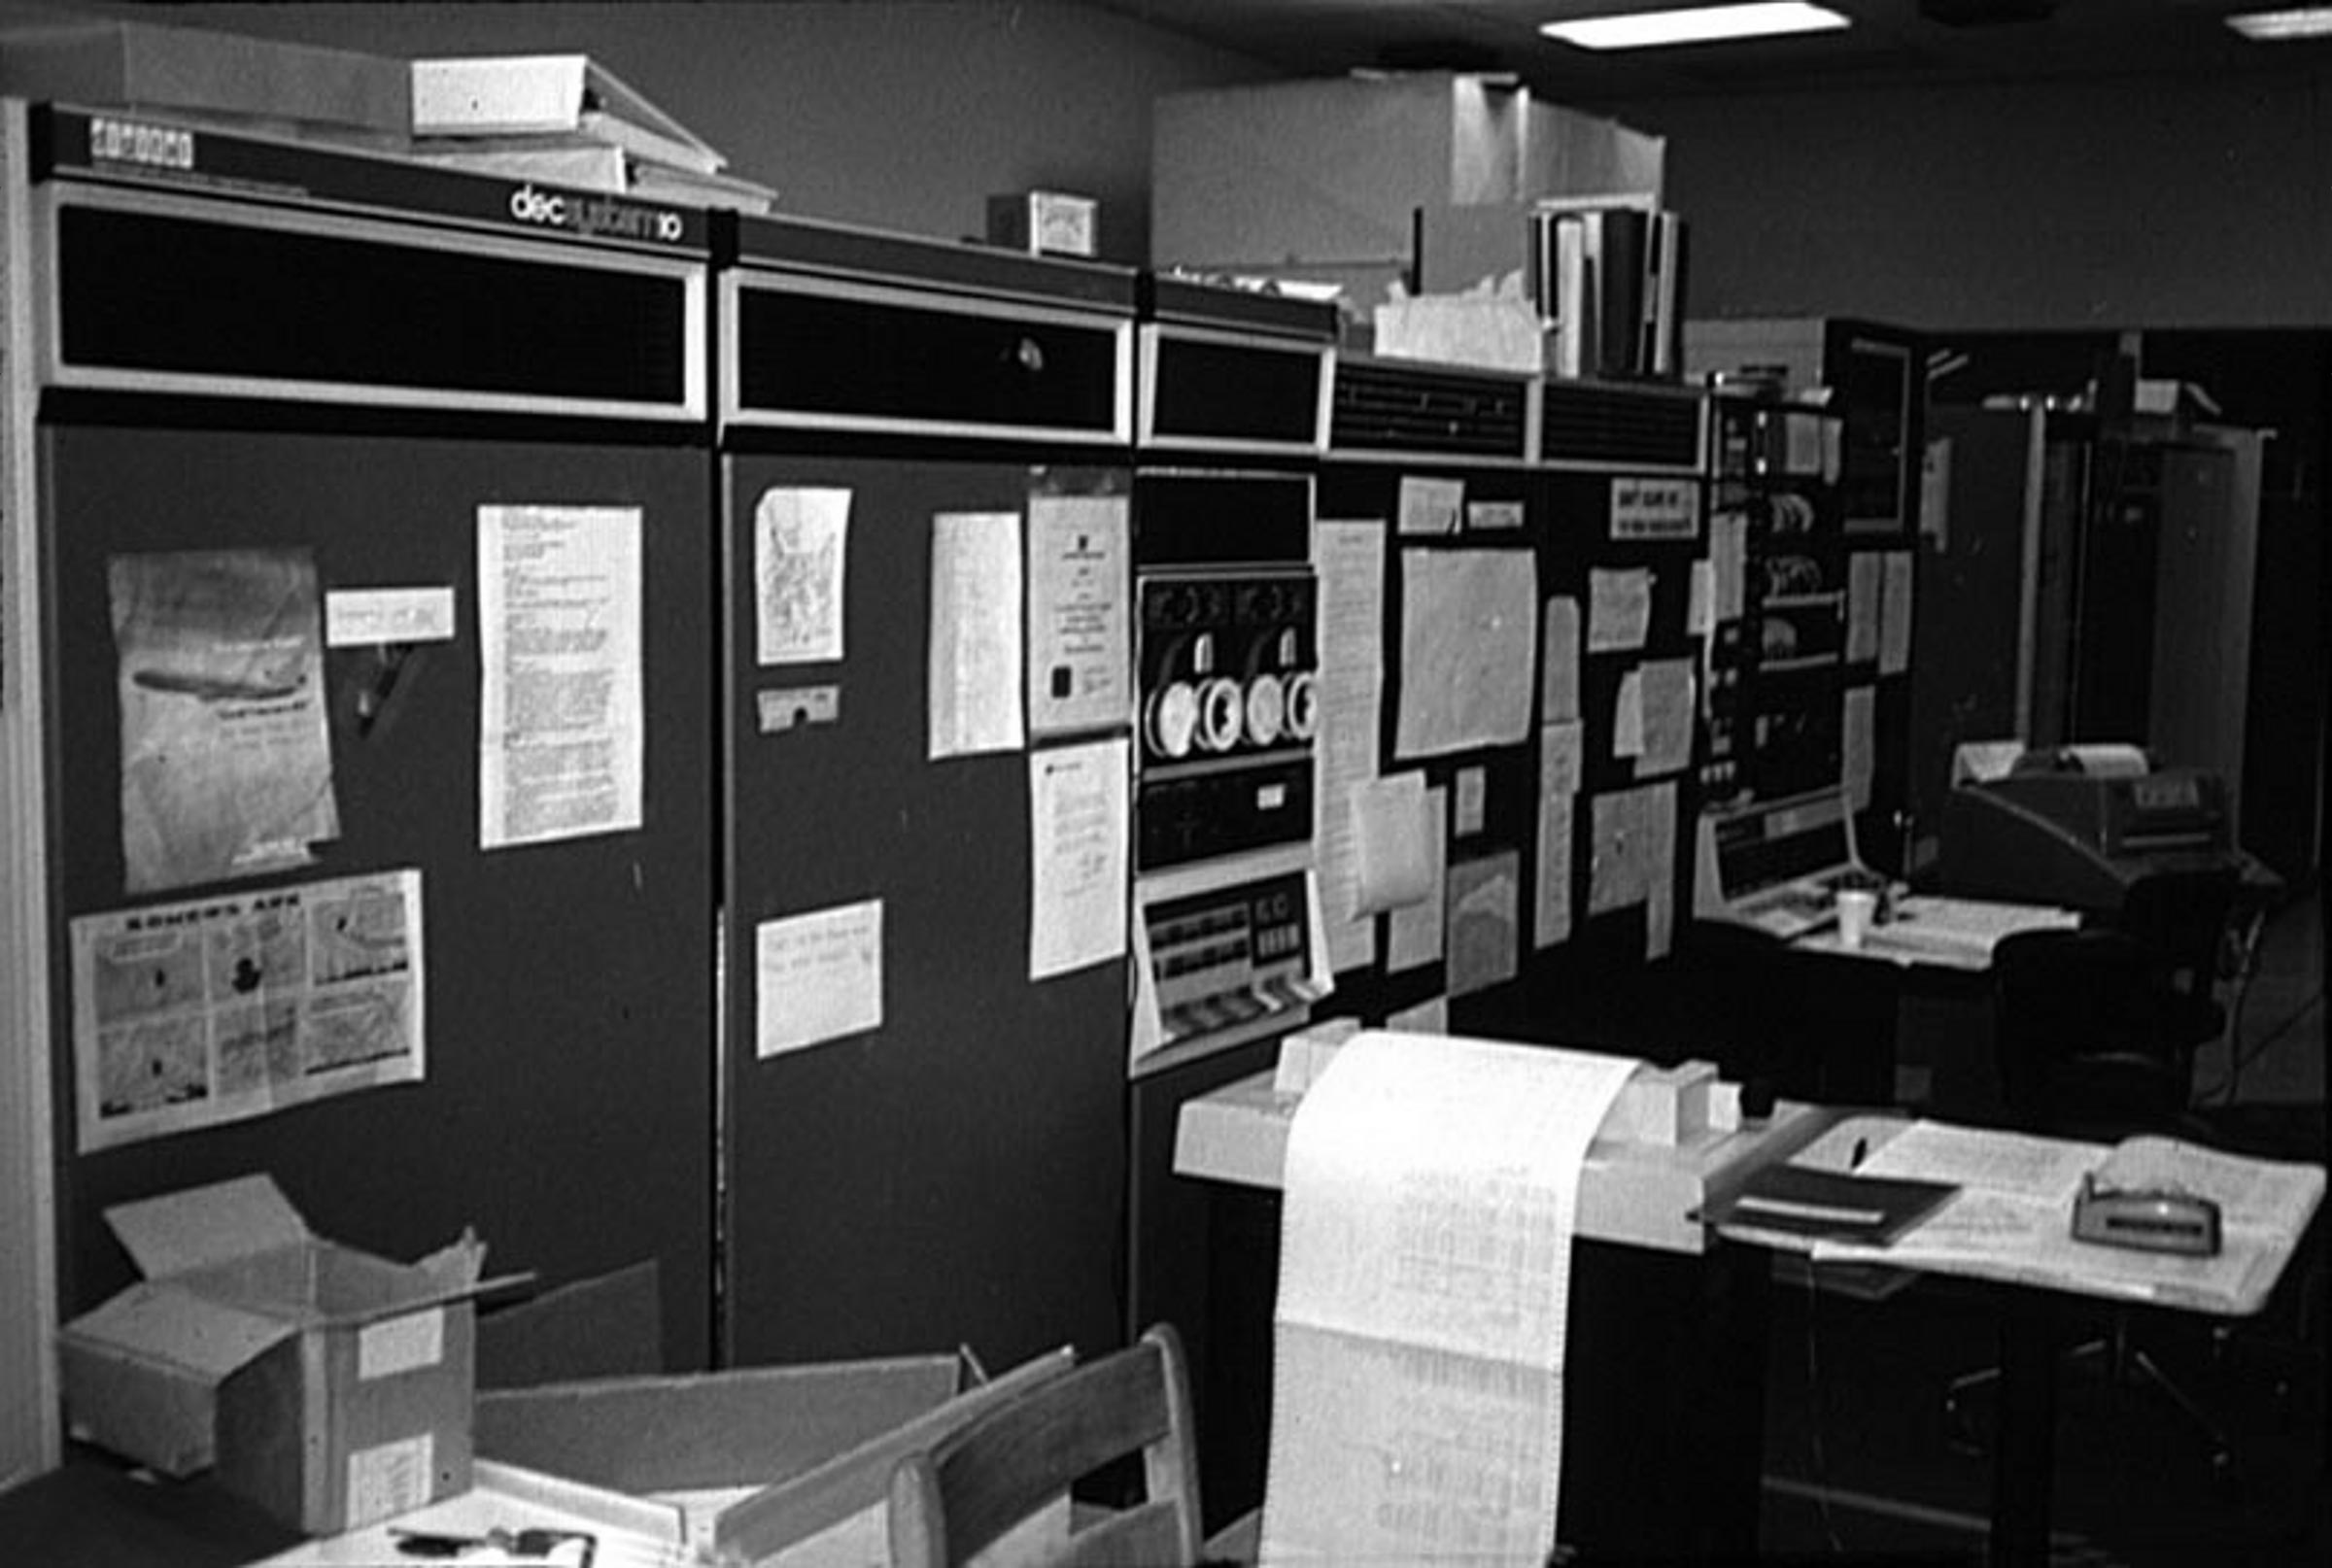
\includegraphics{KL10_1979}
  \caption{PDP-10 processor with KL-10 (a PDP-10 similar to that of the AI Lab), Stanford Artificial Intelligence Laboratory, 1979.}
\end{figure}

``Without hackers to maintain the system, [faculty members] said, `We're going to have a disaster; we must have commercial software,'\hspace{0.01in}'' Stallman would recall a few years later. ``They said, `We can expect the company to maintain it.' It proved that they were utterly wrong, but that's what they did.''\endnote{\textit{Ibid.}}

At first, hackers viewed the Twenex system as yet another authoritarian symbol begging to be subverted. The system's name itself was a protest. Officially dubbed TOPS-20 by DEC, it was named as a successor to TOPS-10, a proprietary operating system DEC distributed for the PDP-10. But TOPS-20 was not based on TOPS-10.  It was derived from the Tenex system which Bolt Beranek Newman had developed for the PDP-10.\endnote{Multiple sources: see Richard Stallman interview, Gerald Sussman email, and \textit{Jargon File 3.0.0} at \url{http://catb.org/jargon/html/T/TWENEX.html}.} Stallman, the hacker who coined the Twenex term, says he came up with the name as a way to avoid using the TOPS-20 name. ``The system was far from tops, so there was no way I was going to call it that,'' Stallman recalls. ``So I decided to insert a `w' in the Tenex name and call it Twenex.''

The machine that ran the Twenex/TOPS-20 system had its own derisive nickname: Oz. According to one hacker legend, the machine got its nickname because it required a smaller PDP-11 machine to power its terminal. One hacker, upon viewing the KL-10-PDP-11 setup for the first time, likened it to the wizard's bombastic onscreen introduction in the Wizard of Oz. ``I am the great and powerful Oz,'' the hacker intoned. ``Pay no attention to the PDP-11 behind that console.''\endnote{See \url{http://www.as.cmu.edu/~geek/humor/See_Figure_1.txt}.}

If hackers laughed when they first encountered the KL-10, their laughter quickly died when they encountered Twenex. Not only did Twenex boast built-in security, but the system's software engineers had designed the tools and applications with the security system in mind. What once had been a cat-and-mouse game over passwords in the case of the Laboratory for Computer Science's security system, now became an out-and-out battle over system management. System administrators argued that without security, the Oz system was more prone to accidental crashes. Hackers argued that crashes could be better prevented by overhauling the source code. Unfortunately, the number of hackers with the time and inclination to perform this sort of overhaul had dwindled to the point that the system-administrator argument prevailed.

The initial policy was that any lab member could have the ``wheel privilege'' to bypass security restrictions.  But anyone who had the ``wheel privilege'' could take it away from anyone else, who would then be powerless to restore it.  This state of affairs tempted a small group of hackers to try to seize total control by canceling the ``wheel privilege'' for all but themselves.

Cadging passwords, and applying the debugger during startup, Stallman successfully foiled these attempts. After the second foiled ``\textit{coup d'état},'' Stallman issued an alert to all the AI Lab personnel.\endnote{See Richard Stallman (1986).}

``There has been another attempt to seize power,'' Stallman wrote. ``So far, the aristocratic forces have been defeated.'' To protect his identity, Stallman signed the message ``Radio Free OZ.''

The disguise was a thin one at best. By 1982, Stallman's aversion to passwords and secrecy had become so well known that users outside the AI Laboratory were using his account from around the ARPAnet -- the research-funded computer network that would serve as a foundation for today's Internet. One such ``tourist'' during the early 1980s was Don Hopkins, a California programmer who learned through the hacking grapevine that all an outsider needed to do to gain access to MIT's vaunted ITS system was to log in under the initials RMS and enter the same three-letter monogram when the system requested a password.

``I'm eternally grateful that MIT let me and many other people use their computers for free,'' says Hopkins. ``It meant a lot to many people.''

This so-called ``tourist'' policy, which had been openly tolerated by MIT management during the ITS years,\endnote{See ``MIT AI Lab Tourist Policy,'' \url{http://www.art.net/~hopkins/Don/text/tourist-policy.html}.} fell by the wayside when Oz became the lab's primary link to the ARPAnet. At first, Stallman continued his policy of repeating his login ID as a password so outside users could have access through his account. Over time, however, Oz's fragility prompted administrators to bar outsiders who, through sheer accident or malicious intent, might bring down the system. When those same administrators eventually demanded that Stallman stop publishing his password, Stallman, citing personal ethics, instead ceased using the Oz system altogether.\endnote{See Richard Stallman (1986).}

``[When] passwords first appeared at the MIT AI Lab I [decided] to follow my belief that there should be no passwords,'' Stallman would later say. ``Because I don't believe that it's really desirable to have security on a computer, I shouldn't be willing to help uphold the security regime.''\endnote{\textit{Ibid.}}

Stallman's refusal to bow before the great and powerful Oz symbolized the growing tension between hackers and AI Lab management during the early 1980s. This tension paled in comparison to the conflict that raged within the hacker community itself. By the time the Decsystem 20 arrived, the hacker community was divided into two camps, LMI and Symbolics.

Symbolics, with its outside investment, recruited various AI Lab hackers and set some of them working on improving parts of the Lisp Machine operating system outside the auspices of the AI Lab. By the end of 1980, the company had hired 14 AI Lab staffers as part-time consultants to develop its version of the Lisp Machine. The remaining few, apart from Stallman, worked for LMI.\endnote{See Steve Levy, \textit{Hackers}, page 423.}  Stallman, preferring the unpressured life at the AI Lab and not wishing to take a side, chose to join neither company.

At first, the other hackers continued spending some of their time at MIT, and contributed to MIT's Lisp Machine operating system. Both LMI and Symbolics had licensed this code from MIT. The license required them to return their changes to MIT, but did not require them to let MIT redistribute these changes.  However, through 1981 they adhered to a gentleman's agreement to permit that, so all their system improvements were included in the MIT version and thus shared with all Lisp Machine users. This situation allowed those still at MIT to remain neutral.

On March 16, 1982, a date Stallman remembers well because it was his birthday, Symbolics executives ended the gentleman's agreement. The motive was to attack LMI. LMI had fewer hackers, and fewer staff in general, so the Symbolics executives thought that LMI was getting the main benefit of sharing the system improvements.  By ending the sharing of system code, they hoped to wipe out LMI.  So they decided to enforce the letter of the license.  Instead of contributing their improvements to the MIT version of the system, which LMI could use, they provided MIT with a copy of the Symbolics version of the system for users at MIT to run.  Anyone using it would provide the service of testing only to Symbolics, and if he made improvements, most likely they too would only be useful for Symbolics.

As the person responsible (with help from Greenblatt for the first couple of months) for keeping up the lab's Lisp Machine system, Stallman was incensed. The Symbolics hackers had left the system code with hundreds of half-made changes that caused errors. Viewing this announcement as an ``ultimatum,'' he retaliated by disconnecting Symbolics' microwave communications link to the laboratory. He then vowed never to work on a Symbolics machine, and pledged to continue the development of MIT's system so as to defend LMI from Symbolics. ``The way I saw it, the AI Lab was a neutral country, like Belgium in World War II,'' Stallman says. ``If Germany invades Belgium, Belgium declares war on Germany and sides with Britain and France.''

When Symbolics executives noticed that their latest features were still appearing in the MIT Lisp Machine system and, by extension, the LMI Lisp machine, they were not pleased. Stallman knew what copyright law required, and was rewriting the features from scratch.  He took advantage of the opportunity to read the source code Symbolics supplied to MIT, so as to understand the problems and fixes, and then made sure to write his changes in a totally different way.  But the Symbolics executives didn't believe this.  They installed a ``spy'' program on Stallman's computer terminal looking for evidence against him.  However, when they took their case to MIT administration, around the start of 1983, they had little evidence to present: a dozen places in the sources where both versions had been changed and appeared similar.

When the AI Lab administrators showed Stallman Symbolics' supposed evidence, he refuted it, showing that the similarities were actually held over from before the fork.  Then he turned the logic around: if, after the thousands of lines he had written, Symbolics could produce no better evidence than this, it demonstrated that Stallman's diligent efforts to avoid copying were effective.  The AI Lab approved Stallman's work, which he continued till the end of 1983.\endnote{\textit{The Brain Makers} by H. P. Newquist says inaccurately that the AI Lab told Stallman to stay away from the Lisp Machine project.}

Stallman did make a change in his practices, though.  ``Just to be ultra safe, I no longer read their source code [for new features and major changes]. I used only the documentation and wrote the code from that.''  For the biggest new features, rather than wait for Symbolics to release documentation, he designed them on his own; later, when the Symbolics documentation appeared, he added compatibility with Symbolics' interface for the feature.  Then he read Symbolics' source code changes to find minor bugs they had fixed, and fixed each of them differently.

The experience solidified Stallman's resolve. As Stallman designed replacements for Symbolics' new features, he also enlisted members of the AI Lab to keep using the MIT system, so as to provide a continuous stream of bug reports. MIT continued giving LMI direct access to the changes. ``I was going to punish Symbolics if it was the last thing I did,'' Stallman says.  Such statements are revealing. Not only do they shed light on Stallman's nonpacifist nature, they also reflect the intense level of emotion triggered by the conflict.

The level of despair owed much to what Stallman viewed as the ``destruction'' of his ``home'' -- i.e., the demise of the AI Lab's close-knit hacker subculture. In a later email interview with Levy, Stallman would liken himself to the historical figure Ishi, the last surviving member of the Yahi, a Pacific Northwest tribe wiped out during the Indian wars of the 1860s and 1870s. The analogy casts Stallman's survival in epic, almost mythical, terms.\endnote{Steven Levy in \textit{Hackers} had this period in mind when he described Stallman as the ``last of the true hackers,'' but his intended meaning was not what you might think.  Levy used the term ``true hackers'' to distinguish the MIT hacker community from two other hacker communities described later in the book, to which he gave other names. When this community had dissolved, leaving only Stallman, he therefore became the last of the ``true hackers.''   Levy did not mean that nobody else was truly a hacker, but people tend to interpret his words that way, especially those who see them without reading the explanations in Levy's book.  Stallman has never described himself using those words of Levy's.} The hackers
who worked for Symbolics saw it differently. Instead of seeing Symbolics as an exterminating force, many of Stallman's colleagues saw it as a belated bid for relevance. In commercializing the Lisp Machine, the company pushed hacker principles of engineer-driven software design out of the ivory-tower confines of the AI Lab and into the corporate marketplace where manager-driven design principles held sway. Rather than viewing Stallman as a holdout, many hackers saw him as the representative of an obsolete practice.

Personal hostilities also affected the situation.   Even before Symbolics hired away most of the AI Lab's hacker staff, Stallman says many of the hackers who later joined Symbolics were shunning him. ``I was no longer getting invited to go to Chinatown,'' Stallman recalls. ``The custom started by Greenblatt was that if you went out to dinner, you went around or sent a message asking anybody at the lab if they also wanted to go. Sometime around 1980-1981, I stopped getting asked. They were not only not inviting me, but one person later confessed that he had been pressured to lie to me to keep their going away to dinner without me a secret.''

Although Stallman felt hurt by this petty form of ostracism, there was nothing to be done about it.  The Symbolics ultimatum changed the matter from a personal rejection to a broader injustice. When Symbolics excluded its source changes from redistribution, as a means to defeat its rival, Stallman determined to thwart Symbolics' goal. By holing up in his MIT offices and writing equivalents for each new software feature and fix, he gave users of the MIT system, including LMI customers, access to the same features as Symbolics users.

It also guaranteed Stallman's legendary status within the hacker community. Already renowned for his work with Emacs, Stallman's ability to match the output of an entire team of Symbolics programmers -- a team that included more than a few legendary hackers itself -- still stands as one of the major human accomplishments of the Information Age, or of any age for that matter. Dubbing it a ``master hack'' and Stallman himself a ``virtual John Henry of computer code,'' author Steven Levy notes that many of his Symbolics-employed rivals had no choice but to pay their idealistic former comrade grudging respect. Levy quotes Bill Gosper, a hacker who eventually went to work for Symbolics in the company's Palo Alto office, expressing amazement over Stallman's output during this period:

\begin{quote}
I can see something Stallman wrote, and I might decide it was bad (probably not, but somebody could convince me it was bad), and I would still say, ``But wait a minute -- Stallman doesn't have anybody to argue with all night over there. He's working alone! It's incredible anyone could do this alone!''\endnote{See Steven Levy, \textit{Hackers} (Penguin USA [paperback], 1984): 426}
\end{quote}

For Stallman, the months spent playing catch up with Symbolics evoke a mixture of pride and profound sadness. As a dyed-in-the-wool liberal whose father had served in World War II, Stallman is no pacifist. In many ways, the Symbolics war offered the rite of passage toward which Stallman had been careening ever since joining the AI Lab staff a decade before. At the same time, however, it coincided with the traumatic destruction of the AI Lab hacker culture that had nurtured Stallman since his teenage years. One day, while taking a break from writing code, Stallman experienced a traumatic moment passing through the lab's equipment room. There, Stallman encountered the hulking, unused frame of the PDP-10 machine. Startled by the dormant lights, lights that once actively blinked out a silent code indicating the status of the internal program, Stallman says the emotional impact was not unlike coming across a beloved family member's well-preserved corpse.

``I started crying right there in the machine room,'' he says. ``Seeing the machine there, dead, with nobody left to fix it, it all drove home how completely my community had been destroyed.''

Stallman would have little opportunity to mourn. The Lisp Machine, despite all the furor it invoked and all the labor that had gone into making it, was merely a sideshow to the large battles in the technology marketplace. The relentless pace of computer miniaturization was bringing in newer, more powerful microprocessors that would soon incorporate the machine's hardware and software capabilities like a modern metropolis swallowing up an ancient desert village.

Riding atop this microprocessor wave were hundreds -- thousands -- of proprietary software programs, each protected by a patchwork of user licenses and nondisclosure agreements that made it impossible for hackers to review or share source code. The licenses were crude and ill-fitting, but by 1983 they had become strong enough to satisfy the courts and scare away would-be interlopers. Software, once a form of garnish most hardware companies gave away to make their expensive computer systems more flavorful, was quickly becoming the main dish. In their increasing hunger for new games and features, users were putting aside the traditional demand to review the recipe after every meal.

Nowhere was this state of affairs more evident than in the realm of personal computer systems. Companies such as Apple Computer and Commodore were minting fresh millionaires selling machines with built-in operating systems. Unaware of the hacker culture and its distaste for binary-only software, many of these users saw little need to protest when these companies failed to attach the accompanying source-code files. A few anarchic adherents of the hacker ethic helped propel that ethic into this new marketplace, but for the most part, the marketplace rewarded the programmers speedy enough to write new programs and savvy enough to write End User License Agreements to lock them up tight.

One of the most notorious of these programmers was Bill Gates, a Harvard dropout two years Stallman's junior. Although Stallman didn't know it at the time, seven years before sending out his message to thenet.unix-wizards newsgroup, Gates, a budding entrepreneur and general partner with the Albuquerque-based software firm Micro-Soft, later spelled as Microsoft, had sent out his own open letter to the software-developer community. Written in response to the PC users copying Micro-Soft's software programs, Gates' ``Open Letter to Hobbyists'' had excoriated the notion of communal software development.

``Who can afford to do professional work for nothing?'' asked Gates. ``What hobbyist can put three man-years into programming, finding all bugs, documenting his product, and distributing it for free?''\endnote{See Bill Gates, ``An Open Letter to Hobbyists'' (February 3, 1976). To view an online copy of this letter, go to \url{http://en.wikipedia.org/wiki/Open_Letter_to_Hobbyists}.}

Although few hackers at the AI Lab saw the missive, Gates' 1976 letter nevertheless represented the changing attitude toward software both among commercial software companies and commercial software developers. Why treat software as a zero-cost commodity when the market said otherwise? As the 1970s gave way to the 1980s, selling software became more than a way to recoup costs; it became a political statement. At a time when the Reagan Administration was rushing to dismantle many of the federal regulations and spending programs that had been built up during the half century following the Great Depression, more than a few software programmers saw the hacker ethic as anticompetitive and, by extension, un-American. At best, it was a throwback to the anticorporate attitudes of the late 1960s and early 1970s. Like a Wall Street banker discovering an old tie-dyed shirt hiding between French-cuffed shirts and double-breasted suits, many computer programmers treated the hacker ethic as an embarrassing reminder of an idealistic age.

For a man who had spent the entire 1960s as a throwback to the 1950s, Stallman didn't mind living out of step with his peers. As a programmer used to working with the best machines and the best software, however, Stallman faced what he could only describe as a ``stark moral choice'': either swallow his ethical objection for ``proprietary'' software -- the term Stallman and his fellow hackers used to describe any program that carried copyright terms or an end-user license that restricted copying and modification -- or dedicate his life to building an alternate, nonproprietary system of software programs. After his two-year battle with Symbolics, Stallman felt confident enough to undertake the latter option. ``I suppose I could have stopped working on computers altogether,'' Stallman says. ``I had no special skills, but I'm sure I could have become a waiter. Not at a fancy restaurant, probably, but I could've been a waiter somewhere.''

Being a waiter -- i.e., dropping out of programming altogether -- would have meant completely giving up an activity, computer programming, that had given him so much pleasure. Looking back on his life since moving to Cambridge, Stallman finds it easy to identify lengthy periods when software programming provided the only pleasure. Rather than drop out, Stallman decided to stick it out.

An Atheist, Stallman rejects notions such as fate, karma, or a divine calling in life. Nevertheless, he does feel that the decision to shun proprietary software and build an operating system to help others do the same was a natural one. After all, it was Stallman's own personal combination of stubbornness, foresight, and coding virtuosity that led him to consider a fork in the road most others didn't know existed. In his article, ``The GNU Project,'' Stallman affirms agreement with the ideals encapsulated in the words of the Jewish sage Hillel:

\begin{quote}
If I am not for myself, who will be for me? If I am only for myself, what am I? If not now, when?\endnote{See \url{http://www.gnu.org/gnu/the-gnu-project.html}. Stallman adds his own footnote to this statement, writing, ``As an Atheist, I don't follow any religious leaders, but I sometimes find I admire something one of them has said.''}
\end{quote}

Speaking to audiences, Stallman avoids the religious route and expresses the decision in pragmatic terms. ``I asked myself: what could I, an operating-system developer, do to improve the situation? It wasn't until I examined the question for a while that I realized an operating-system developer was exactly what was needed to solve the problem.''

Once he recognized that, Stallman says, everything else ``fell into place.'' In 1983, MIT was acquiring second-generation Lisp Machines from Symbolics, on which the MIT Lisp Machine system could not possibly run.  Once most of the MIT machines were replaced, he would be unable to continue maintaining that system effectively for lack of users' bug reports.  He would have to stop.  But he also wanted to stop.  The MIT Lisp Machine system was not free software: even though users could get the source code, they could not redistribute it freely.  Meanwhile, the goal of continuing the MIT system had already been achieved: LMI had survived and was developing software on its own.

Stallman didn't want to spend his whole life punishing those who had destroyed his old community.  He wanted to build a new one. He decided to denounce software that would require him to compromise his ethical beliefs, and devote his life to the creation of programs that would make it easier for him and others to escape from it. Pledging to build a free software operating system ``or die trying -- of old age, of course,'' Stallman quips, he resigned from the MIT staff in January, 1984, to build GNU.

The resignation distanced Stallman's work from the legal auspices of MIT. Still, Stallman had enough friends and allies within the AI Lab to continue using the facilities, and later his own office. He also had the ability to secure outside consulting gigs to underwrite the early stages of the GNU Project. In resigning from MIT, however, Stallman negated any debate about conflict of interest or Institute ownership of the software. The man whose early adulthood fear of social isolation had driven him deeper and deeper into the AI Lab's embrace was now building a legal firewall between himself and that environment.

For the first few months, Stallman operated in isolation from the Unix community as well. Although his announcement to the net.unix-wizards group had attracted sympathetic responses, few volunteers signed on to join the crusade in its early stages.

``The community reaction was pretty much uniform,'' recalls Rich Morin, leader of a Unix user group at the time. ``People said, `Oh, that's a great idea. Show us your code. Show us it can be done.'\hspace{0.01in}''

Aware that the job was enormous, Stallman decided to try to reuse existing free software wherever possible.  So he began looking for existing free programs and tools that could be converted into GNU programs and tools. One of the first candidates was a compiler named VUCK, which converted programs written in the popular C programming language into machine-runnable code. Translated from the Dutch, the program's acronym stood for the Free University Compiler Kit. Optimistic, Stallman asked the program's author if the program was free. When the author informed him that the words ``Free University'' were a reference to the Vrije Universiteit in Amsterdam, and that the program was not free, Stallman was chagrined.

``He responded derisively, stating that the university was free but the compiler was not,'' recalls Stallman. He had not only refused to help -- he suggested Stallman drop his plan to develop GNU, and instead write some add-ons to boost sales of VUCK, in return for a share of the profits. ``I therefore decided that my first program for the GNU Project would be a multi-language, multi-platform compiler.''\endnote{See Richard Stallman, ``The GNU Operating System and the Free Software Movement,'' \textit{Open Sources} (O'Reilly \& Associates, Inc., 1999): 65.}

Instead of VUCK, Stallman found the Pastel compiler (``off-color Pascal''), written by programmers at Lawrence Livermore National Lab. According to what they said when they gave him a copy, the compiler was free to copy and modify. Unfortunately, the program was unsuitable for the job, because its memory requirements were enormous.  It parsed the entire input file in core memory, then retained all the internal data until it finished compiling the file. On mainframe systems this design had been forgivable. On Unix systems it was a crippling barrier, since even 32-bit machines that ran Unix were often unable to provide so much memory to a program. Stallman made substantial progress at first, building a C-compatible frontend to the compiler and testing it on the larger Vax, whose system could handle large memory spaces. When he tried porting the system to the 68010, and investigated why it crashed,  he discovered the memory size problem, and concluded he would have to build a totally new compiler from scratch.  Stallman eventually did this, producing the GNU C Compiler or GCC.  But it was not clear in 1984 what to do about the compiler, so he decided to let those plans gel while turning his attention to other parts of GNU.

In September of 1984, thus, Stallman began development of a GNU version of Emacs, the replacement for the program he had been supervising for a decade. Within the Unix community, the two native editor programs were vi, written by Sun Microsystems cofounder Bill Joy, and ed, written by Bell Labs scientist (and Unix cocreator) Ken Thompson. Both were useful and popular, but neither offered the endlessly expandable nature of Emacs.

Looking back, Stallman says he didn't view the decision in strategic terms. ``I wanted an Emacs, and I had a good opportunity to develop one.''

Once again, Stallman had found existing code with which he hoped to save time. In writing a Unix version of Emacs, Stallman was soon following the footsteps of Carnegie Mellon graduate student James Gosling, author of a C-based version dubbed Gosling Emacs or Gosmacs. Gosling's version of Emacs included an interpreter for a simplified offshoot of the Lisp language, called Mocklisp. Although Gosling had put Gosmacs under copyright and had sold the rights to UniPress, a privately held software company, Stallman received the assurances of a fellow developer who had participated in early Gosmacs development. According to the developer, Gosling, while a Ph.D. student at Carnegie Mellon, had given him permission by email to distribute his own version of Gosmacs in exchange for his contribution to the code.

At first Stallman thought he would change only the user-level commands, to implement full compatibility with the original PDP-10 Emacs.  However, when he found how weak Mocklisp was in comparison with real Lisp, he felt compelled to replace it with a true Lisp system.  This made it natural to rewrite most of the higher-level code of Gosmacs in a completely different way, taking advantage of the greater power and flexible data structures of Lisp.  By mid-1985, in GNU Emacs as released on the Internet, only a few files still had code remaining from Gosmacs.

Then UniPress caught wind of Stallman's project, and denied that the other developer had received permission to distribute his own version of Gosmacs.  He could not find a copy of the old email to defend his claim.  Stallman eliminated this problem by writing replacements for the few modules that remained from Gosmacs.

Nevertheless, the notion of developers selling off software rights -- indeed, the very notion of developers having such powers to sell in the first place -- rankled Stallman. In a 1986 speech at the Swedish Royal Technical Institute, Stallman cited the UniPress incident as yet another example of the dangers associated with proprietary software.

``Sometimes I think that perhaps one of the best things I could do with my life is find a gigantic pile of proprietary software that was a trade secret, and start handing out copies on a street corner so it wouldn't be a trade secret any more,'' said Stallman. ``Perhaps that would be a much more efficient way for me to give people new free software than actually writing it myself; but everyone is too cowardly to even take it.''\endnote{See Richard Stallman (1986).}

Despite the stress it generated, the dispute over Gosling's code would assist both Stallman and the free software movement in the long term. It would force Stallman to address the weaknesses of the Emacs Commune and the informal trust system that had allowed problematic offshoots to emerge. It would also force Stallman to sharpen the free software movement's political objectives. Following the release of GNU Emacs in 1985, Stallman issued \textit{The GNU Manifesto}, an expansion of the original announcement posted in September, 1983. Stallman included within the document a lengthy section devoted to the many arguments used by commercial and academic programmers to justify the proliferation of proprietary software programs. One argument, ``Don't programmers deserve a reward for their creativity,'' earned a response encapsulating Stallman's anger over the recent Gosling Emacs episode:

``If anything deserves a reward, it is social contribution,'' Stallman wrote. ``Creativity can be a social contribution, but only in so far [\textit{sic}] as society is free to use the results. If programmers deserve to be rewarded for creating innovative programs, by the same token they deserve to be punished if they restrict the use of these programs.''\endnote{See Richard Stallman, \textit{The GNU Manifesto} (1985), \url{http://www.gnu.org/gnu/manifesto.html}.}

With the release of GNU Emacs, the GNU Project finally had code to show. It also had the burdens of any software-based enterprise. As more and more Unix developers began playing with the software, money, gifts, and requests for tapes began to pour in. To address the business side of the GNU Project, Stallman drafted a few of his colleagues and formed the Free Software Foundation (FSF), a nonprofit organization dedicated to speeding the GNU Project towards its goal. With Stallman as president and various friends and hacker allies as board members, the FSF helped provide a corporate face for the GNU Project.

Robert Chassell, a programmer then working at Lisp Machines, Inc., became one of five charter board members at the Free Software Foundation following a dinner conversation with Stallman. Chassell also served as the organization's treasurer, a role that started small but quickly grew.

``I think in '85 our total expenses and revenue were something in the order of \$23,000, give or take,'' Chassell recalls. ``Richard had his office, and we borrowed space. I put all the stuff, especially the tapes, under my desk. It wasn't until sometime later LMI loaned us some space where we could store tapes and things of that sort.''

In addition to providing a face, the Free Software Foundation provided a center of gravity for other disenchanted programmers. The Unix market that had seemed so collegial even at the time of Stallman's initial GNU announcement was becoming increasingly competitive. In an attempt to tighten their hold on customers, companies were starting to deny users access to Unix source code, a trend that only speeded the number of inquiries into ongoing GNU software projects. The Unix wizards who once regarded Stallman as a noisy kook were now beginning to see him as a software prophet or a software Cassandra, according as they felt hope or despair over escaping the problems he identified.

``A lot of people don't realize, until they've had it happen to them, how frustrating it can be to spend a few years working on a software program only to have it taken away,'' says Chassell, summarizing the feelings and opinions of the correspondents writing in to the FSF during the early years. ``After that happens a couple of times, you start to say to yourself, `Hey, wait a minute.'\hspace{0.01in}''

For Chassell, the decision to participate in the Free Software Foundation came down to his own personal feelings of loss. Prior to LMI, Chassell had been working for hire, writing an introductory book on Unix for Cadmus, Inc., a Cambridge-area software company. When Cadmus folded, taking the rights to the book down with it, Chassell says he attempted to buy the rights back with no success.

``As far as I know, that book is still sitting on a shelf somewhere, unusable, uncopyable, just taken out of the system,'' Chassell says. ``It was quite a good introduction if I may say so myself. It would have taken maybe three or four months to convert [the book] into a perfectly usable introduction to GNU/Linux today. The whole experience, aside from what I have in my memory, was lost.''

Forced to watch his work sink into the mire while his erstwhile employer struggled through bankruptcy, Chassell says he felt a hint of the anger that drove Stallman to fits of apoplexy. ``The main clarity, for me, was the sense that if you want to have a decent life, you don't want to have bits of it closed off,'' Chassell says. ``This whole idea of having the freedom to go in and to fix something and modify it, whatever it may be, it really makes a difference. It makes one think happily that after you've lived a few years that what you've done is worthwhile. Because otherwise it just gets taken away and thrown out or abandoned or, at the very least, you no longer have any relation to it. It's like losing a bit of your life.''

\bigskip

\theendnotes
\setcounter{endnote}{0}
